\documentclass[border=12pt]{standalone}
\usepackage{tikz}
\usetikzlibrary{shapes.geometric, arrows.meta, positioning, calc, fit, backgrounds}
\usepackage{fontspec}
\usepackage{amsmath,amssymb}
\setmainfont{DejaVu Sans}

\begin{document}
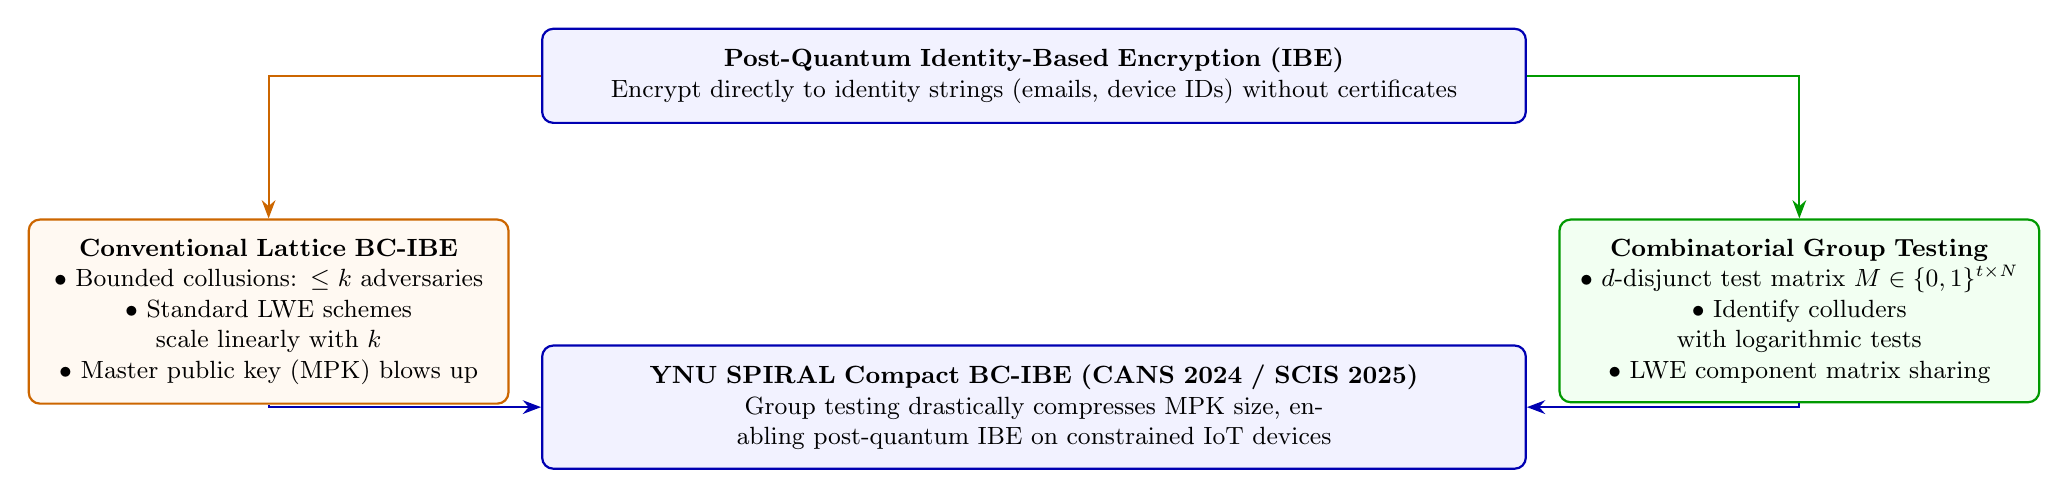
\begin{tikzpicture}[
    font=\small,
    >=Stealth,
    node distance=1.2cm,
    block/.style={rectangle, draw=blue!70!black, fill=blue!5, rounded corners=4pt, thick, align=center, inner sep=7pt},
    alertblock/.style={rectangle, draw=red!70!black, fill=red!5, rounded corners=4pt, thick, align=center, inner sep=7pt},
    greenblock/.style={rectangle, draw=green!60!black, fill=green!5, rounded corners=4pt, thick, align=center, inner sep=7pt},
    amberblock/.style={rectangle, draw=orange!80!black, fill=orange!5, rounded corners=4pt, thick, align=center, inner sep=7pt}
]

\node[block, text width=12cm] (top) {\textbf{Post-Quantum Identity-Based Encryption (IBE)}\\Encrypt directly to identity strings (emails, device IDs) without certificates};

\node[amberblock, below left=1.2cm and 0.4cm of top, text width=5.6cm] (bottleneck) {\textbf{Conventional Lattice BC-IBE}\\$\bullet$ Bounded collusions: $\le k$ adversaries\\$\bullet$ Standard LWE schemes scale linearly with $k$\\$\bullet$ Master public key (MPK) blows up};

\node[greenblock, below right=1.2cm and 0.4cm of top, text width=5.6cm] (grouptest) {\textbf{Combinatorial Group Testing}\\$\bullet$ $d$-disjunct test matrix $M \in \{0, 1\}^{t \times N}$\\$\bullet$ Identify colluders with logarithmic tests\\$\bullet$ LWE component matrix sharing};

\node[block, below=2.8cm of top, text width=12cm] (bottom) {\textbf{YNU SPIRAL Compact BC-IBE (CANS 2024 / SCIS 2025)}\\Group testing drastically compresses MPK size, enabling post-quantum IBE on constrained IoT devices};

\draw[->, thick, orange!80!black] (top) -| (bottleneck);
\draw[->, thick, green!60!black] (top) -| (grouptest);
\draw[->, thick, blue!70!black] (bottleneck) |- (bottom);
\draw[->, thick, blue!70!black] (grouptest) |- (bottom);

\end{tikzpicture}
\end{document}
